%%%%%%%%%%%%%%%%%%%%%%%%%%%%%%%%%%%%%%%%%
% Beamer Presentation
% LaTeX Template
% Version 1.0 (10/11/12)
%
% This template has been downloaded from:
% http://www.LaTeXTemplates.com
%
% License:
% CC BY-NC-SA 3.0 (http://creativecommons.org/licenses/by-nc-sa/3.0/)
%
%%%%%%%%%%%%%%%%%%%%%%%%%%%%%%%%%%%%%%%%%

%----------------------------------------------------------------------------------------
%   PACKAGES AND THEMES
%----------------------------------------------------------------------------------------

%\documentclass[trans]{beamer}
\documentclass{beamer}

\mode<presentation> {

\usetheme{CambridgeUS}

}

\usepackage{graphicx} % Allows including images
\usepackage{booktabs} % Allows the use of \toprule, \midrule and \bottomrule in tables
\usepackage{pgf}
\usepackage{import}

\usepackage{xcolor}
\usepackage{tabularx}
\renewcommand\tabularxcolumn[1]{m{#1}}
\newcolumntype{L}{>{\raggedright\arraybackslash}X}

\usepackage{multicol}
\usepackage{multirow}

\usepackage{tikz}
\usetikzlibrary{positioning}

\definecolor{normalbg}{HTML}{EDF2FC}
\definecolor{normalfg}{HTML}{012528}
\definecolor{normalsymbol}{HTML}{012528}

\definecolor{examplebg}{HTML}{1098F7}%{A76571}%
\definecolor{alertbg}{HTML}{FAC05E}
\definecolor{myblue}{HTML}{DA4167}

\definecolor{blue}{HTML}{264653}
\definecolor{green}{HTML}{2a9d8f}
\definecolor{yellow}{HTML}{e9c46a}
\definecolor{orange}{HTML}{f4a261}
\definecolor{red}{HTML}{e76f51}

\setbeamercolor{normal text}{fg=normalfg,bg=white}
\setbeamercolor{alerted text}{fg=normalfg,bg=alertbg}
\setbeamercolor{example text}{fg=normalfg,bg=examplebg}

\setbeamercolor{background canvas}{fg=normalfg,bg=white}
\setbeamercolor{background}{fg=black,bg=white}

\setbeamercolor{palette primary}{fg=normalfg, bg=normalbg}
\setbeamercolor{palette secondary}{fg=normalfg, bg=alertbg}
\setbeamercolor{palette tertiary}{fg=normalfg, bg=examplebg}

\setbeamercolor{block title}{fg=normalfg,bg=normalbg}
\setbeamertemplate{itemize item}{\color{normalfg}$\blacksquare$}
\setbeamertemplate{itemize subitem}{\color{normalfg}$\blacktriangleright$}

\setbeamercolor{frametitle}{fg=normalfg,bg=normalbg}
\setbeamercolor{title}{fg=normalfg,bg=normalbg}

%----------------------------------------------------------------------------------------
%   TITLE PAGE
%----------------------------------------------------------------------------------------

\title[SAT Competition 2022]{The Results of SAT Competition 2022}

\author[Balyo, Heule, Iser, J\"{a}rvisalo, Suda] {Tom{\'a}{\v s} Balyo, Marijn Heule,
{\bf Markus Iser},\\ Matti J\"{a}rvisalo, and Martin Suda}
\institute[] % Your institution as it will appear on the bottom of every slide, may be shorthand to save space
{
SAT 2022 Conference, Haifa (Israel) \\ % Your institution for the title page
}
\date{August 5, 2022} % Date, can be changed to a custom date

\begin{document}

\begin{frame}
\titlepage % Print the title page as the first slide
\end{frame}

\begin{frame}{Competition Anniversary}

\begin{block}{Anniversary of SAT Competitions}
\begin{itemize}
\item 3 competitions in the 90s\hfill (1992,1993, 1996)
\item 14 SAT Competitions \hfill (2002--)
\item 5 SAT Races \hfill (2006, 2008, 2010, 2015, 2019)
\item 1 SAT Challenge \hfill (2012)
\end{itemize}
\end{block}

\bigskip

\begin{block}{Goals}
\begin{itemize}
\item Promotion of SAT solvers and their development
\item Compilation of new challenging benchmarks
\item Evaluation of current state-of-the-art solvers
\end{itemize}
\end{block}

\end{frame}


\begin{frame}{Key rules}
\begin{itemize}
\item Certified results of unsatisfiability using DRAT proof logging
  \begin{itemize}
  \item Instance is ``not solved'' if proof checker finds inconsistency in proof
  \end{itemize}
\medskip
\item Disqualification of buggy solvers
  \begin{itemize}
  \item Producing an incorrect model
  \item Report UNSAT on a known satisfiable instance
  \end{itemize}
\medskip
\item Mandatory solver descriptions + open source
\medskip
\item Ranking scheme: PAR-2
\begin{itemize}
\item Favors solvers that are faster (not only count solved instances)
\end{itemize}
\medskip
\item BYOB (Bring Your Own Benchmarks)
\begin{itemize}
\item At most 20 instances per participant are used
\end{itemize} 
\end{itemize}
\end{frame}


\begin{frame}{Competition Summary}
\begin{block}{Main Track}
\begin{itemize}
  \item 400 benchmarks (300 new submission, 100 of previous competitions)
  \item 52 sequential solvers
  \item 10 parallel solvers
  \item 2 cloud solvers
\end{itemize}
\end{block}

\begin{block}{Anniversary Track (20 years of SAT competition)}
\begin{itemize}
  \item 5355 benchmarks (all past application/crafted/main tracks)
  \item 29 sequential solvers
  \item 6 parallel solvers
  \item 2 cloud solvers
\end{itemize}
\end{block}
\end{frame}


\begin{frame}{Anniversary Track}
\begin{block}{Track Data}
\begin{itemize}\setlength\itemsep{1em}
\item Large Dataset: 5355 benchmarks $\times$ 37 solvers
\item Subject to Post-Competition Analysis
\item Will be published at Zenodo
\item In this Competition: Pandas saved my life!
\begin{itemize}\setlength\itemsep{.5em}
\item 1 TB of Competition Data 
\item 827 LoC for Aggregation and Analysis
\end{itemize}
\end{itemize}
\end{block}
\end{frame}


\begin{frame}{Anniversary Cloud Track}
\begin{block}{Winning Solvers}\centering
\begin{tabularx}{\linewidth}{clLrrc}
& \bf Solver & \bf Authors & \bf PAR-2 & \bf Solved & \\ \hline
1 & Mallob-KiCaLiGlu & Dominik Schreiber & 279.27 & 4687 & \\ 
2 & Paracooba & Maximilian Heisinger & 725.07 & 3619 & \\ 
\end{tabularx}
\end{block}

\begin{block}{Results for Satisfiable Instances (Claimed SAT)}\centering
\color{normalfg!50}
\begin{tabularx}{\linewidth}{clLrrc}
& \bf Solver & \bf Authors & \bf PAR-2 & \bf Solved & \\ \hline
1 & Mallob-KiCaLiGlu & Dominik Schreiber & 34.57 & 2170 & \\ 
2 & Paracooba & Maximilian Heisinger & 411.18 & 1808 & \\ 
\end{tabularx}
\end{block}

\begin{block}{Results for Unsatisfiable Instances (Claimed UNSAT)}\centering
\color{normalfg!50}
\begin{tabularx}{\linewidth}{clLrrc}
& \bf Solver & \bf Authors & \bf PAR-2 & \bf Solved & \\ \hline
1 & Mallob-KiCaLiGlu & Dominik Schreiber & 56.85 & 2517 & \\ 
2 & Paracooba & Maximilian Heisinger & 674.69 & 1811 & \\ 
\end{tabularx}
\end{block}
\end{frame}

\begin{frame}{Anniversary Cloud Track}
\centering
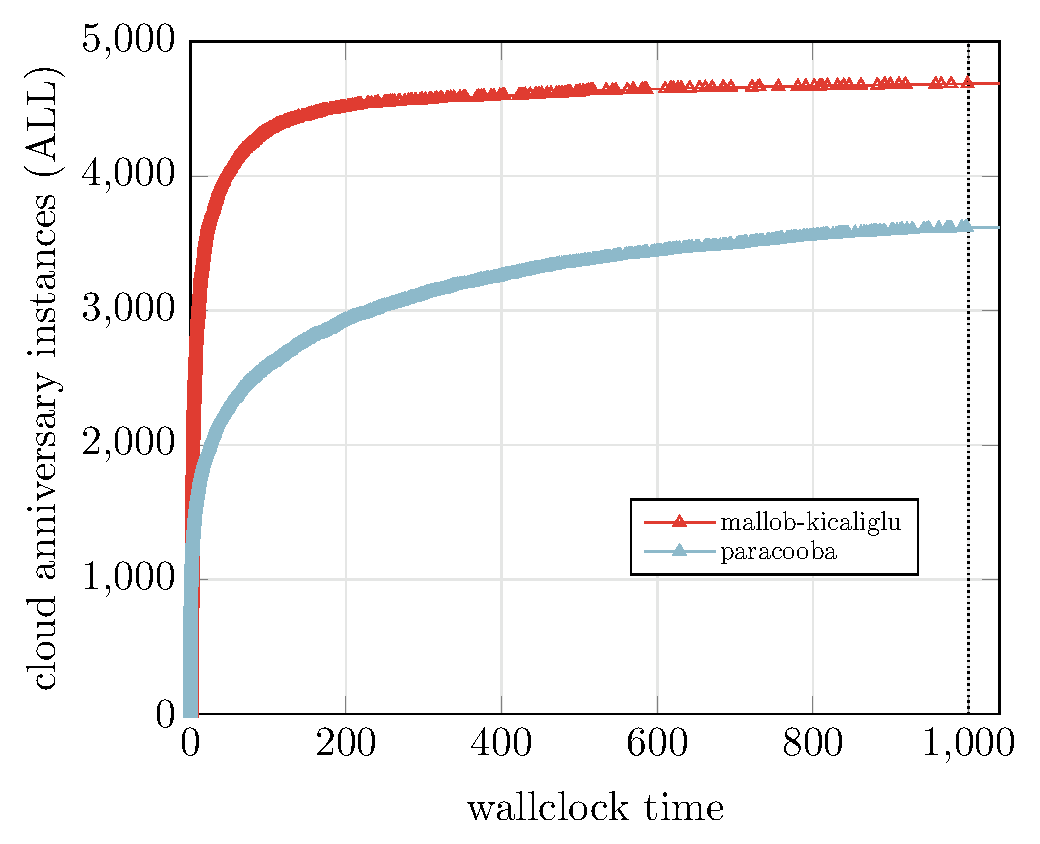
\includegraphics[width=.8\linewidth]{plots/cloud-anni-2022.pdf}
\end{frame}


\begin{frame}{Anniversary Parallel Track SAT}
\begin{block}{Winning Solvers}\centering
\renewcommand{\arraystretch}{2}
\begin{tabularx}{\linewidth}{clLrrc}
& \bf Solver & \bf Authors & \bf PAR-2 & \bf Solved & \\ \hline
1 & Mergesat-aws & Norbert Manthey & 890.65 & 2047 & \\ 
2 & Mallob-Ki & Dominik Schreiber & 927.81 & 2031 & \\ 
3 & DPS & Hidetomo Nabeshima, Tsubasa Fukiage, Yuto Obitsu, Xiao-Nan Lu, and Katsumi Inoue & 1586.13 & 1911 & \\ 
\end{tabularx}
\end{block}
\end{frame}

\begin{frame}{Anniversary Parallel Track UNSAT}
\begin{block}{Winning Solvers}\centering
\renewcommand{\arraystretch}{2}
\begin{tabularx}{\linewidth}{clLrrc}
& \bf Solver & \bf Authors & \bf PAR-2 & \bf Solved & \\ \hline
1 & Mallob-Ki & Dominik Schreiber & 893.52 & 2369 & \\ 
2 & Mergesat-aws & Norbert Manthey & 2400.30 & 2029 & \\ 
3 & DPS & Hidetomo Nabeshima, Tsubasa Fukiage, Yuto Obitsu, Xiao-Nan Lu, and Katsumi Inoue & 2881.27 & 1925 & \\ 
\end{tabularx}
\end{block}
\end{frame}

\begin{frame}{Anniversary Parallel Track}
\begin{block}{Winning Solvers}\centering
\renewcommand{\arraystretch}{2}
\begin{tabularx}{\linewidth}{clLrrc}
& \bf Solver & \bf Authors & \bf PAR-2 & \bf Solved & \\ \hline
1 & Mallob-Ki & Dominik Schreiber & 1992.46 & 4400 & \\ 
2 & Mergesat-aws & Norbert Manthey & 2689.75 & 4076 & \\ 
3 & DPS & Hidetomo Nabeshima, Tsubasa Fukiage, Yuto Obitsu, Xiao-Nan Lu, and Katsumi Inoue & 3200.95 & 3836 & \\ 
\end{tabularx}
\end{block}
\end{frame}

\begin{frame}{Anniversary Parallel Track}
\centering
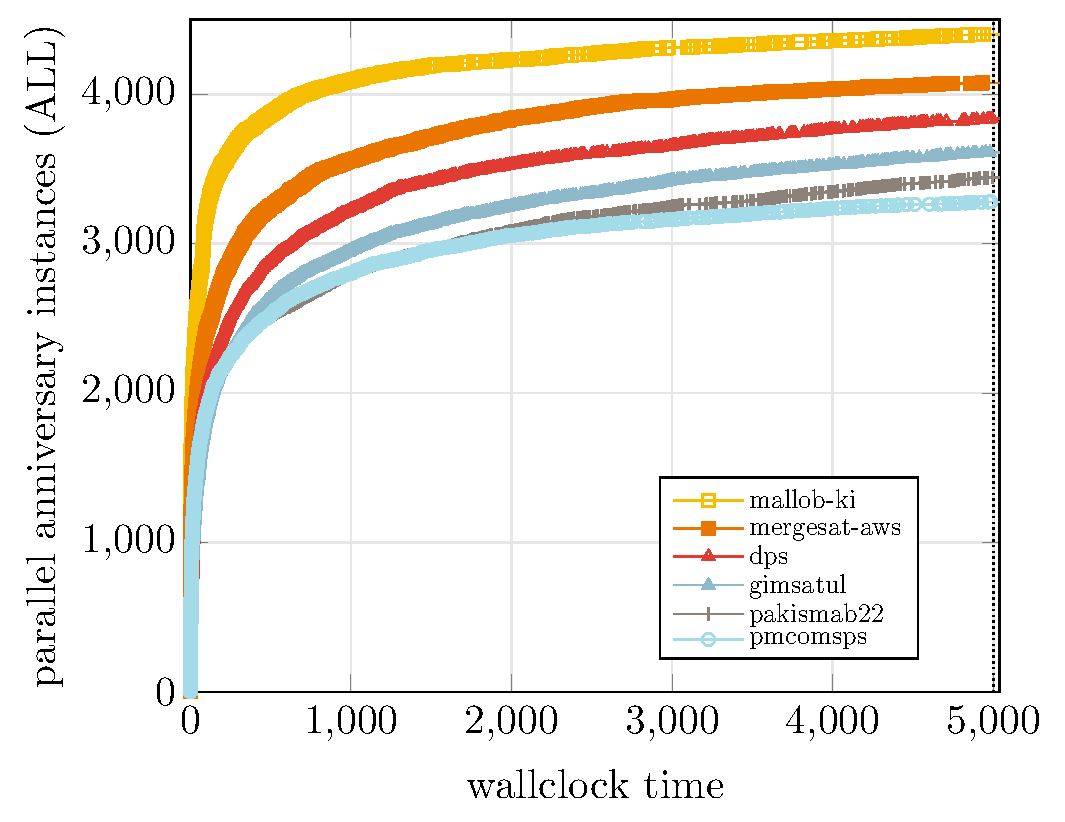
\includegraphics[width=.8\linewidth]{plots/parallel-anni-2022.pdf}
\end{frame}


\begin{frame}{Anniversary Sequential Track SAT}
\begin{block}{Winning Solvers}\centering
\renewcommand{\arraystretch}{2}
\begin{tabularx}{\linewidth}{clLrrc}
& \bf Solver & \bf Authors & \bf PAR-2 & \bf Solved & \\ \hline
1 & Kissat-sc2022-bulky & Armin Biere and Mathias Fleury & 1161.18 & 1962 & \\ 
2 & Kissat-MAB-UCB & Mohamed Sami Cherif, Djamal Habet, and Cyril Terrioux & 1168.71 & 1949 & \\ 
3 & eKissat-MAB-gb-db & Md Solimul Chowdhury & 1168.76 & 1947 & \\ 
\end{tabularx}
\end{block}
\end{frame}

\begin{frame}{Anniversary Sequential Track UNSAT}
\begin{block}{Winning Solvers}\centering
\renewcommand{\arraystretch}{1.7}
\begin{tabularx}{\linewidth}{clLrrc}
& \bf Solver & \bf Authors & \bf PAR-2 & \bf Solved & \\ \hline
1 & hKis-unsat & Rodrigue Konan Tchinda and Clementin Tayou Djamegni & 1071.99 & 2080 & \\ 
2 & Kissat-MAB-ESA & Shuolin Li, Jordi Coll, Chu-Min Li, Mao Luo, Djamal Habet, and Felip Manyà & 1093.82 & 2078 & \\ 
3 & Kissat-sc2022-bulky & Armin Biere and Mathias Fleury & 1115.26 & 2076 & \\ 
\end{tabularx}
\end{block}
\end{frame}

\begin{frame}{Anniversary Sequential Track}
\begin{block}{Winning Solvers}\centering
\renewcommand{\arraystretch}{2}
\begin{tabularx}{\linewidth}{clLrrc}
& \bf Solver & \bf Authors & \bf PAR-2 & \bf Solved & \\ \hline
1 & Kissat-MAB-ESA & Shuolin Li, Jordi Coll, Chu-Min Li, Mao Luo, Djamal Habet, and Felip Manyà & 2806.15 & 4029 & \\ 
2 & Kissat-sc2022-bulky & Armin Biere and Mathias Fleury & 2810.70 & 4038 & \\ 
3 & eKissat-MAB-gb-db & Md Solimul Chowdhury & 2829.88 & 4015 & \\ 
\end{tabularx}
\end{block}
\end{frame}

\begin{frame}{Anniversary Sequential Track}
\centering
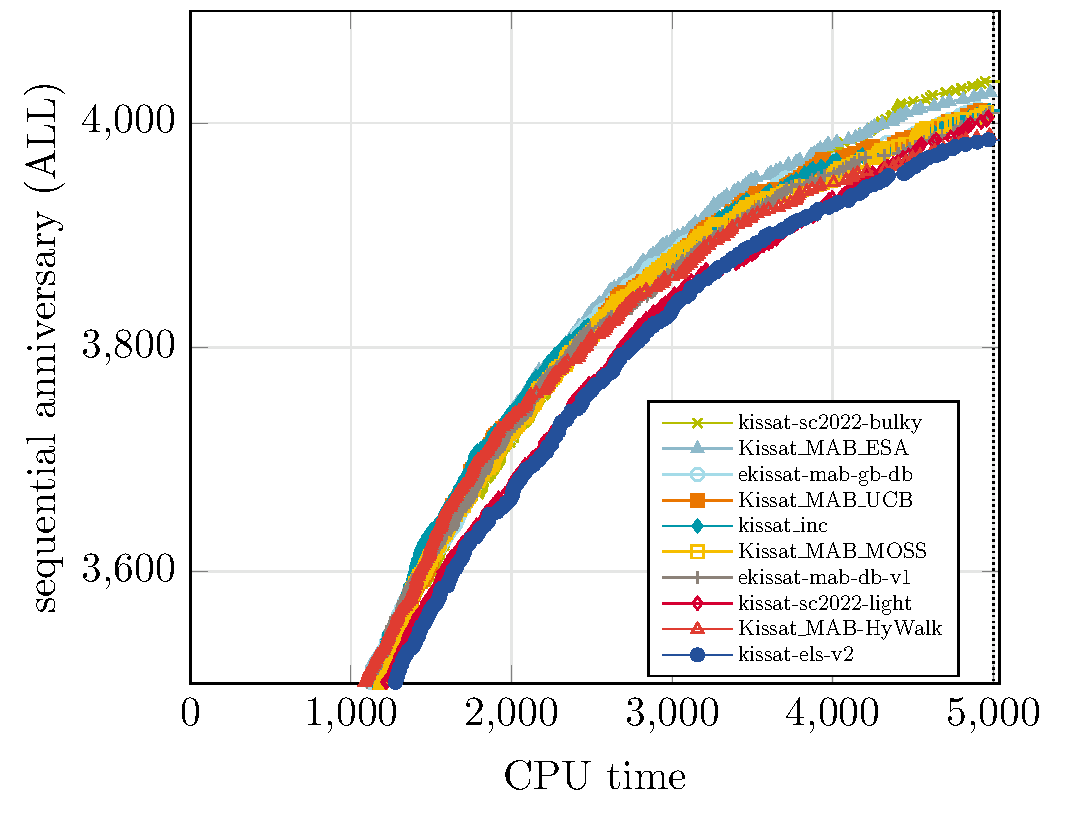
\includegraphics[width=.8\linewidth]{plots/seq10-anni-2022.pdf}
\end{frame}

\begin{frame}{Anniversary Track Winners: Sequential, Parallel, Cloud}
\centering
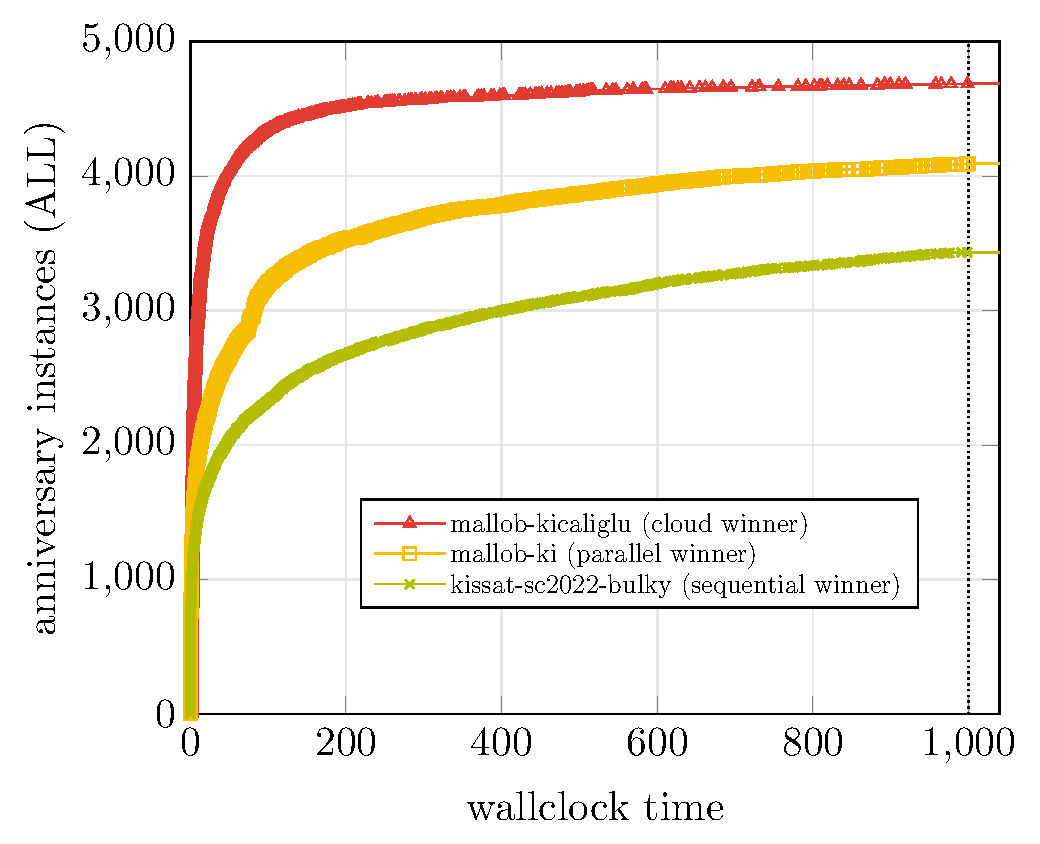
\includegraphics[width=.8\linewidth]{plots/cloud-par-seq-anni-2022.pdf}
\end{frame}


\begin{frame}{Main Cloud Track}
\begin{block}{Winning Solvers}\centering
\begin{tabularx}{\linewidth}{clLrrc}
& \bf Solver & \bf Authors & \bf PAR-2 & \bf Solved & \\ \hline
1 & Mallob-KiCaLiGlu & Dominik Schreiber & 344.78 & 341 & \\ 
2 & Paracooba & Maximilian Heisinger & 1025.51 & 221 & \\ 
\end{tabularx}
\end{block}

\begin{block}{Results for Satisfiable Instances (Claimed SAT)}\centering
\color{normalfg!50}
\begin{tabularx}{\linewidth}{clLrrc}
& \bf Solver & \bf Authors & \bf PAR-2 & \bf Solved & \\ \hline
1 & Mallob-KiCaLiGlu & Dominik Schreiber & 108.36 & 165 & \\ 
2 & Paracooba & Maximilian Heisinger & 795.02 & 111 & \\ 
\end{tabularx}
\end{block}

\begin{block}{Results for Unsatisfiable Instances (Claimed UNSAT)}\centering
\color{normalfg!50}
\begin{tabularx}{\linewidth}{clLrrc}
& \bf Solver & \bf Authors & \bf PAR-2 & \bf Solved & \\ \hline
1 & Mallob-KiCaLiGlu & Dominik Schreiber & 179.48 & 176 & \\ 
2 & Paracooba & Maximilian Heisinger & 1012.13 & 110 & \\ 
\end{tabularx}
\end{block}
\end{frame}

\begin{frame}{Main Cloud Track}
\centering
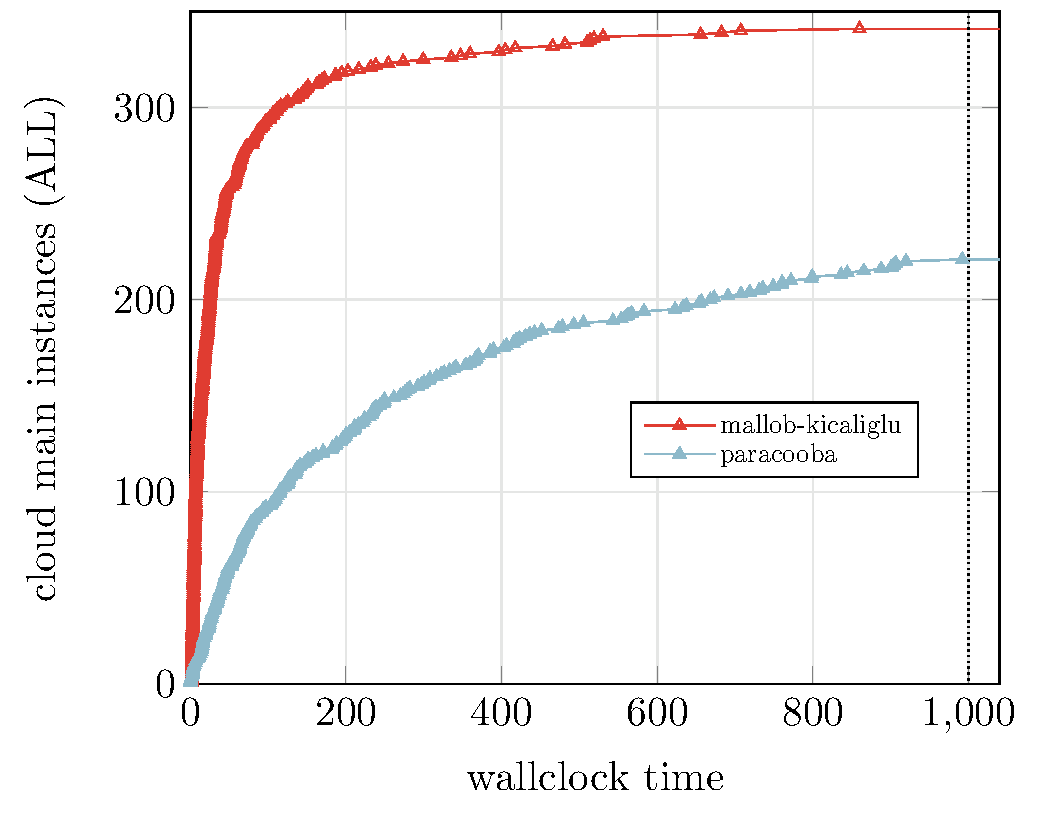
\includegraphics[width=.8\linewidth]{plots/cloud-main-2022.pdf}
\end{frame}


\begin{frame}{Main Parallel Track SAT}
\begin{block}{Winning Solvers}\centering
\renewcommand{\arraystretch}{2}
\begin{tabularx}{\linewidth}{clLrrc}
& \bf Solver & \bf Authors & \bf PAR-2 & \bf Solved & \\ \hline
1 & parKissat-rs & Xindi Zhang, Zhihan Chen, and Shaowei Cai & 654.27 & 163 & \\[1em]
\multirow{2}{*}{2} & DPS & \multirow{2}{=}{Hidetomo Nabeshima, Tsubasa Fukiage, Yuto Obitsu, Xiao-Nan Lu, and Katsumi Inoue} & 1445.86 & 153 & \\ 
 & NPS &  & 1448.02 & 152 & \\
3 & PaKis22 & Rodrigue Konan Tchinda, Clémentin Tayou Djamegni & 1838.79 & 148
\end{tabularx}
\end{block}
\end{frame}

\begin{frame}{Main Parallel Track UNSAT}
\begin{block}{Winning Solvers}\centering
\renewcommand{\arraystretch}{2}
\begin{tabularx}{\linewidth}{clLrrc}
& \bf Solver & \bf Authors & \bf PAR-2 & \bf Solved & \\ \hline
1 & Mallob-Ki & Dominik Schreiber & 1597.21 & 163 & \\ 
2 & parKissat-rs & Xindi Zhang, Zhihan Chen, and Shaowei Cai & 1613.96 & 163 & \\ 
3 & NPS & Hidetomo Nabeshima, Tsubasa Fukiage, Yuto Obitsu, Xiao-Nan Lu, and Katsumi Inoue & 2377.65 & 151 & \\ 
\end{tabularx}
\end{block}
\end{frame}

\begin{frame}{Main Parallel Track}
\begin{block}{Winning Solvers}\centering
\renewcommand{\arraystretch}{2}
\begin{tabularx}{\linewidth}{clLrrc}
& \bf Solver & \bf Authors & \bf PAR-2 & \bf Solved & \\ \hline
1 & parKissat-rs & Xindi Zhang, Zhihan Chen, and Shaowei Cai & 2105.19 & 326 & \\ 
\multirow{2}{*}{2} & NPS & \multirow{2}{=}{Hidetomo Nabeshima, Tsubasa Fukiage, Yuto Obitsu, Xiao-Nan Lu, and Katsumi Inoue} & 2799.64 & 303 & \\ 
 & DPS &  & 2799.72 & 305 & \\ 
3 & Mallob-Ki & Dominik Schreiber & 2987.64 & 292 & 
\end{tabularx}
\end{block}
\end{frame}

\begin{frame}{Main Parallel Track}
\centering
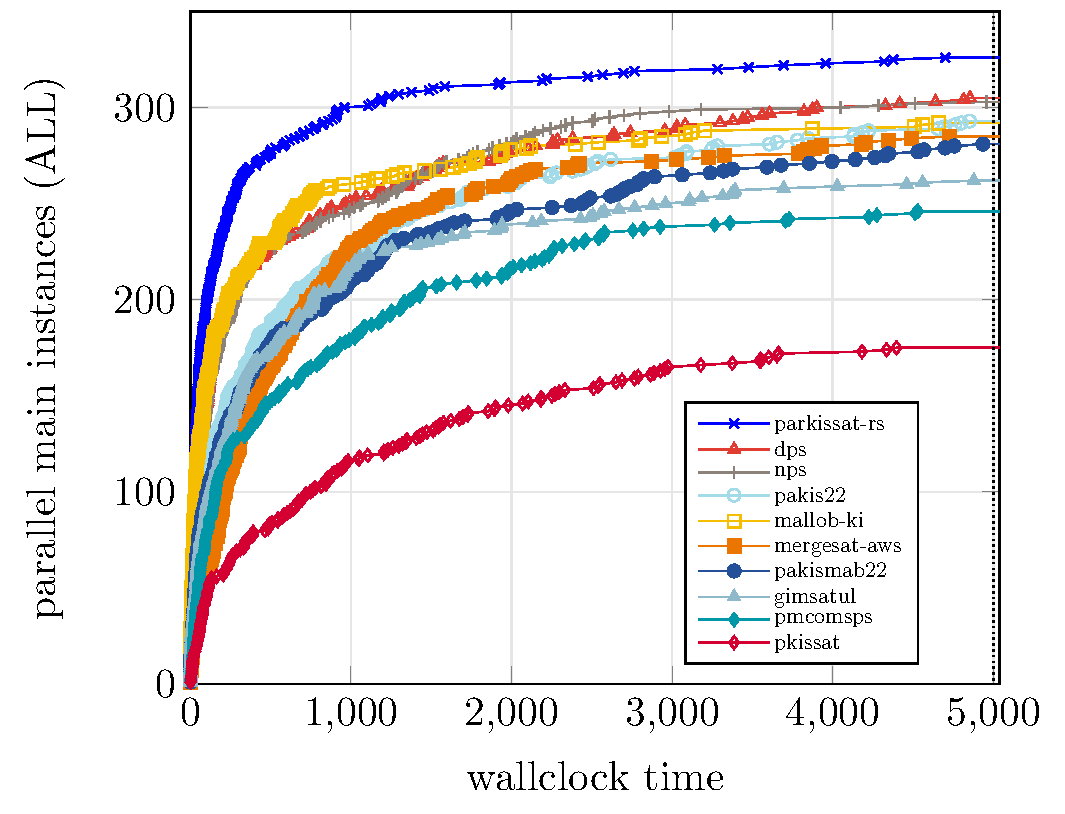
\includegraphics[width=.8\linewidth]{plots/parallel-main-2022.pdf}
\end{frame}


\begin{frame}{Main Sequential Track SAT}
\begin{block}{Winning Solvers}\centering
\renewcommand{\arraystretch}{1.6}
\begin{tabularx}{\linewidth}{clLrrc}
& \bf Solver & \bf Authors & \bf PAR-2 & \bf Solved & \\ \hline
\multirow{2}{*}{1} & SeqFROST-NoExtend & \multirow{2}{=}{Muhammad Osama and Anton Wijs} & 1709.42 & 144 & \\ 
 & SeqFROST-ERE-All &  & 1715.51 & 144 & \\ 
2 & Kissat-inc & Zhihan Chen, Xindi Zhang, Shaowei Cai, and Pinyan Lu & 1769.02 & 145 & \\ 
3 & Kissat-MAB-HyWalk & Jiongzhi Zheng, Kun He, Zhuo Chen, Jianrong Zhou, and Chu-Min Li & 1779.61 & 144 &
\end{tabularx}
\end{block}
\end{frame}

\begin{frame}{Main Sequential Track UNSAT}
\begin{block}{Winning Solvers}\centering
\renewcommand{\arraystretch}{2}
\begin{tabularx}{\linewidth}{clLrrc}
& \bf Solver & \bf Authors & \bf PAR-2 & \bf Solved & \\ \hline
\multirow{2}{*}{1} & hKis-psids & \multirow{2}{=}{Rodrigue Konan Tchinda and Clementin Tayou Djamegni} & 1284.38 & 150 & \\ 
  & hKis-unsat &  & 1484.25 & 145 & \\ 
2 & Kissat-sc2022-bulky & Armin Biere and Mathias Fleury & 1471.83 & 149 & \\ 
3 & Kissat-MAB-UCB & Mohamed Sami Cherif, Djamal Habet and Cyril Terrioux & 1524.93 & 147
\end{tabularx}
\end{block}
\end{frame}

\begin{frame}{Main Sequential Track}
\begin{block}{Winning Solvers}\centering
\renewcommand{\arraystretch}{1.7}
\begin{tabularx}{\linewidth}{clLrrc}
& \bf Solver & \bf Authors & \bf PAR-2 & \bf Solved & \\ \hline
1 & Kissat-MAB-HyWalk & Jiongzhi Zheng, Kun He, Zhuo Chen, Jianrong Zhou, and Chu-Min Li & 3334.22 & 290 & \\ 
\multirow{2}{*}{2} & Kissat-inc & \multirow{2}{=}{Zhihan Chen, Xindi Zhang, Shaowei Cai, and Pinyan Lu} & 3351.93 & 290 & \\ 
 & Kissat-pre &  & 3380.17 & 288 & \\ 
3 & eKissat-MAB-db-v1 & Md Solimul Chowdhury & 3402.95 & 287 &  
\end{tabularx}
\end{block}
\end{frame}

\begin{frame}{Main Sequential Track}
\centering
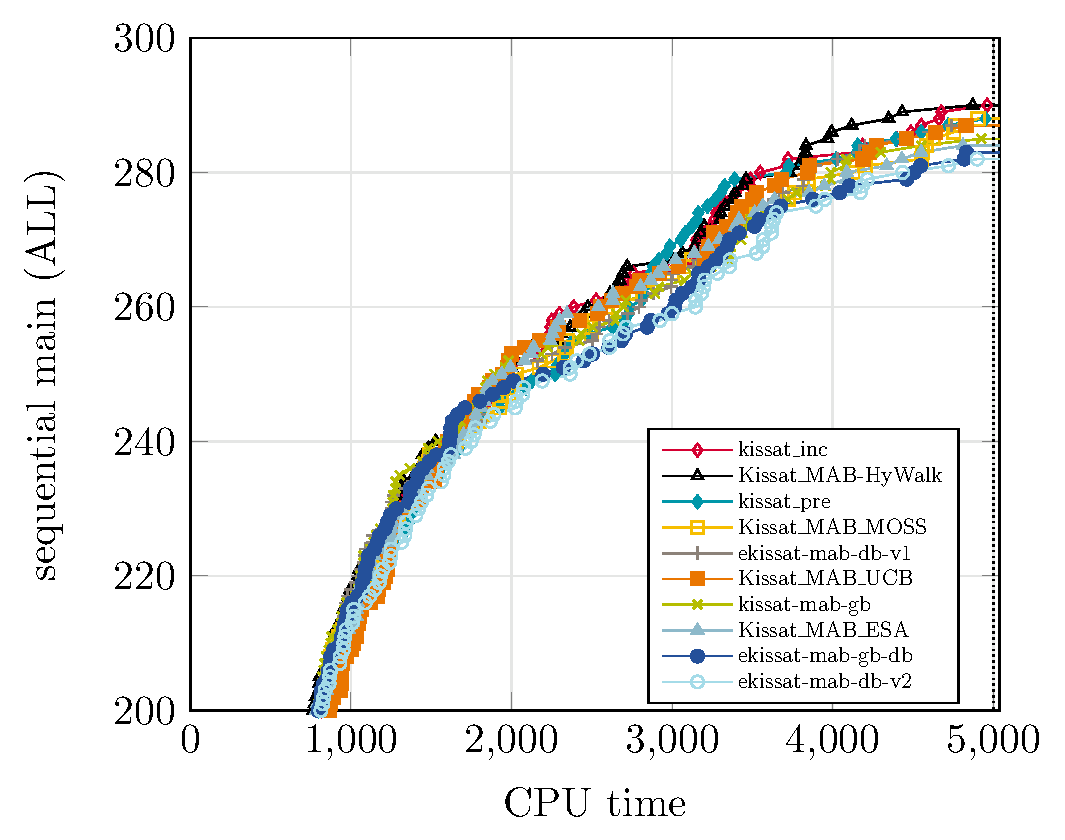
\includegraphics[width=.8\linewidth]{plots/seq10-main-2022.pdf}
\end{frame}


\begin{frame}{Main Track Winners: Sequential, Parallel, Cloud}
\centering
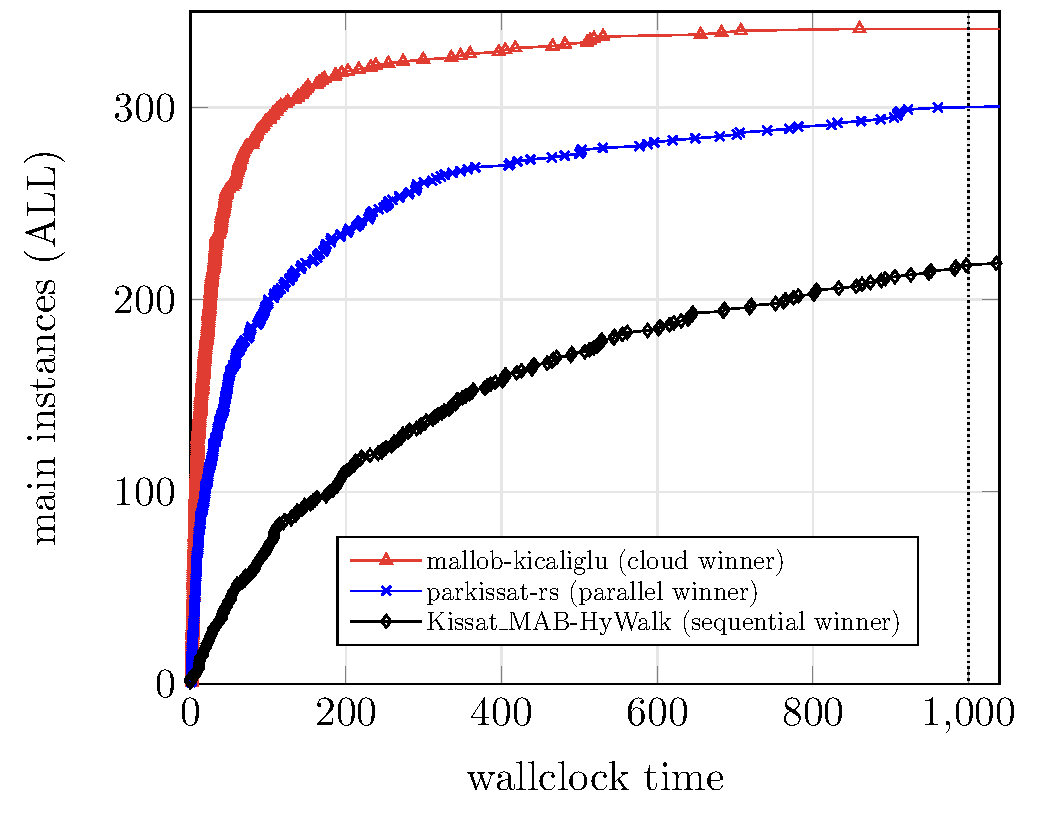
\includegraphics[width=.8\linewidth]{plots/cloud-par-seq-main-2022.pdf}
\end{frame}


\begin{frame}{Issues in 2022}
\begin{block}{Certificates}
\centering

\begin{itemize}\setlength\itemsep{1em}
	\item Rules do not cover corner cases, esp. for UNSAT certificates
	\begin{itemize}
		\item Wrong Proofs
		\item Proof Checker Timeouts (45k seconds)
	\end{itemize}
	\item Not an issue for the top solvers
	\item \emph{This will change for 2023}\\[1em]
\begin{tabular}{cc|ccc}
Result & Certificate & SAT & UNSAT (2022) & UNSAT (2023) \\
\hline
Wrong & Wrong & Disq. & Disq. & Disq. \\
Correct & Timeout & Disq. & Solved & \bf Unsolved \\
Correct & Wrong & Disq. & Unsolved & \bf Disq. \\
\end{tabular}
\end{itemize}
\end{block}
\end{frame}

\begin{frame}{UNSAT Certificates for Parallel Solvers}
\begin{block}{UNSAT proof certificates will be enforced "sooner than you think"}
	\begin{itemize}\setlength\itemsep{1em}
		\item 2022: notable correctness issues with parallel solvers
		\item \emph{2023 will see a new track (per discussions at PoS 2022)}\\[.5em]
		\begin{itemize}\setlength\itemsep{1em}
			\item Incentives for developing proof certification for parallel SAT solvers
			\item (Perhaps not in 2023 though\dots but soon enough!)
		\end{itemize}
	\end{itemize}
\end{block}
\end{frame}

\begin{frame}{New for 2023: Open Call for Proof Checkers}
\begin{block}{Support More Powerful Proof Systems}
\begin{itemize}\setlength\itemsep{.5em}
\item Call to be released by early September
\item Intent to submit (incl. extended abstract): early fall
\item Submission deadline: November 30, 2022 (preliminary)
\item Checkers announced by January 15, 2023 (preliminary)
\item \textbf{Requirement:} Checkers must be \emph{formally verified}
\item Main track UNSAT
\item \textbf{Implications:}
\begin{itemize}
\item Each solver must specify checker  be used to check its proofs
\item Per-instance time limit on proof checking 
\item "Solving" an instance requires that  proof can be checked 
\end{itemize}
\end{itemize}
\end{block}
\end{frame}

\begin{frame}{New for 2023: Challenge Track (preliminarily planned)}
\begin{block}{Large Anniversary Track Dataset}
\begin{itemize}\setlength\itemsep{1em}
\item Benchmark set public 
\item Benchmarks: unsolved instances from the 2022 Anniversary track
\item \textbf{Challenge:} Devise a SAT solver which can solve as many of the benchmark instances
\begin{itemize}\setlength\itemsep{1em}
\item "Solved": solved sequentially on StarExec within the 2022 Anniversary track time limit
\item Results checked by organizers
\item "Hall of fame": list for each instance authors who solved it and when was the certificate submitted
\end{itemize}
\end{itemize}
\end{block}
\end{frame}


\begin{frame}{Thank you!}
\begin{center}
\begin{tikzpicture}[fill=normalbg]
\node[xshift=-2em] (aws) at (current page.north west) { 
\includegraphics[width=13em]{img/AWSlogo.png} };
\node[xshift=-18em] (cas) at (current page.north east) { 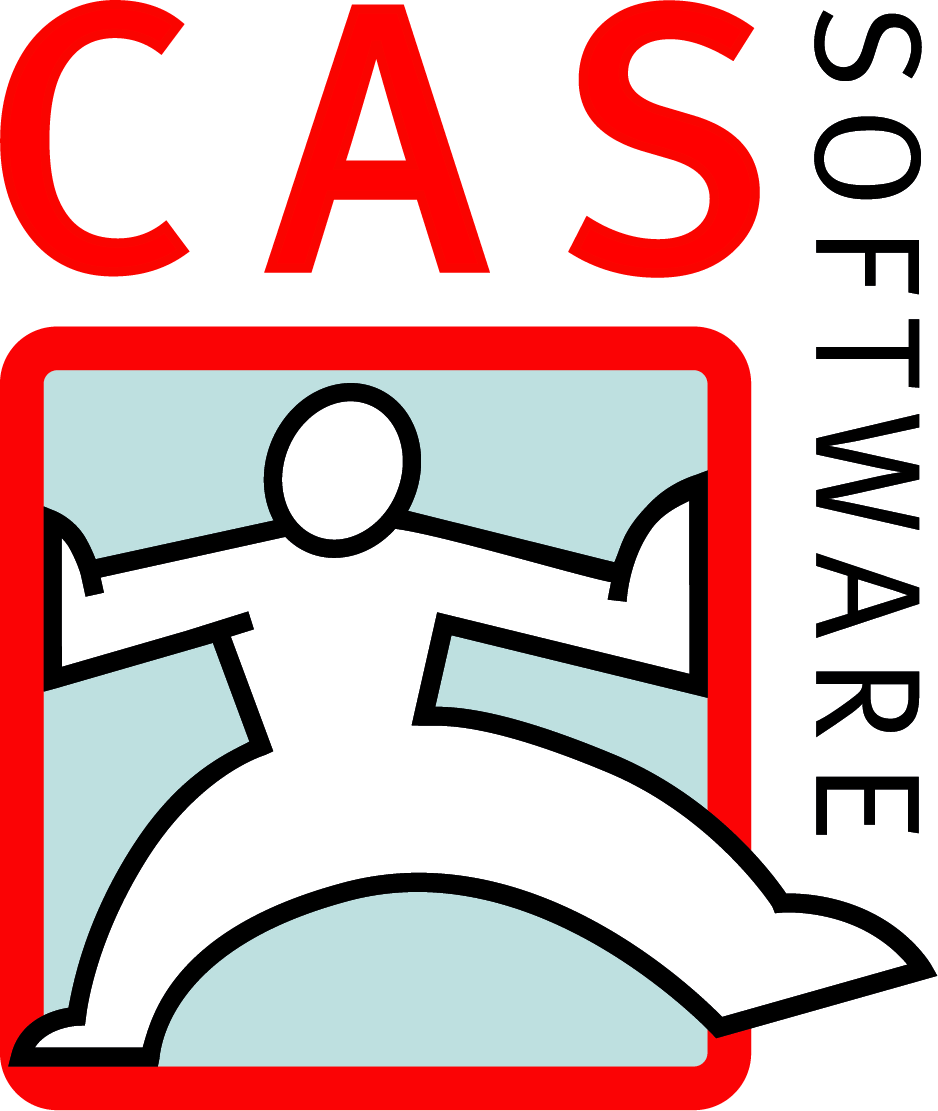
\includegraphics[width=8em]{img/CASlogo.png} };
\node[fill=black, xshift=5em, yshift=15em] (sex) at (current page.south west) { 
\includegraphics[width=20em]{img/SEXlogo.png} };
\end{tikzpicture}
\end{center}
\end{frame}


%----------------------------------------------------------------------------------------

\end{document}